\lab{The QR Decomposition}{The QR Decomposition}
\label{lab:QRdecomp}
\objective{The QR decomposition is a fundamentally important matrix factorization.
It is straightforward to implement, is numerically stable, and provides the basis of several important algorithms.
In this lab we explore several ways to produce the QR decomposition and implement a few immediate applications.
% \\ \indent We restrict our discussion to real matrices.
% However, the results and algorithms presented here can be extended to complex matrices by replacing ``transpose'' with ``hermitian conjugate'' and ``symmetric matrix'' with ``hermitian matrix.''
}

The QR decomposition of a matrix $A$ is a factorization $A=QR$, where $Q$ is  has orthonormal columns and $R$ is upper triangular.
Every $m \times n$ matrix $A$ of rank $n \le m$ has a QR decomposition, with two main forms.
%
\begin{itemize}
    \item \textbf{Reduced QR}: $Q$ is $m \times n$, $R$ is $n \times n$, and the columns $\{\q_j\}_{j=1}^n$ of $Q$ form an orthonormal basis for the column space of $A$.
    \item \textbf{Full QR}: $Q$ is $m \times m$ and $R$ is $m \times n$.
    In this case, the columns $\{\q_j\}_{j=1}^m$ of $Q$ form an orthonormal basis for all of $\mathbb{F}^m$, and the last $m - n$ rows of $R$ only contain zeros.
    If $m = n$, this is the same as the reduced factorization.
\end{itemize}
We distinguish between these two forms by writing $\widehat{Q}$ and $\widehat{R}$ for the reduced decomposition and $Q$ and $R$ for the full decomposition.
%
\begin{align*} % Reduced and full QR decompositions.
\begin{array}{ccc}
\textcolor{red}{\widehat{Q}\ (m \times n)} & \textcolor{blue}{\widehat{R}\ (n \times n)} & \\
\left[\begin{array}{cccccccc}
\arrayrulecolor{red}
\cline{2-4}
& \lvl{}     &        & \rvl{}     &          &        &      & \\
& \lvl{}     &        & \rvl{}     &          &        &      & \\
& \lvl{}     &        & \rvl{}     &          &        &      & \\
& \lvl{\q_1} & \cdots & \rvl{\q_n} & \q_{n+1} & \cdots & \q_m & \\
& \lvl{}     &        & \rvl{}     &          &        &      & \\
& \lvl{}     &        & \rvl{}     &          &        &      & \\
& \lvl{}     &        & \rvl{}     &          &        &      & \\
\cline{2-4}
\end{array}\right]
&
\left[\begin{array}{ccccc}
\arrayrulecolor{blue}
\cline{2-4}
& \lvl{r_{11}} & \cdots & \rvl{r_{1n}} & \\
& \lvl{}       & \ddots & \rvl{\vdots} & \\
& \lvl{}       &        & \rvl{r_{nn}} & \\
\cline{2-4}
& 0            & \cdots & 0            & \\
& \vdots       &        & \vdots       & \\
& 0            & \cdots & 0            & \\
\end{array}\right]
& =\ A\ (m \times n)
\\
Q\ (m \times m) & R\ (m \times n) & \\
\end{array}
\end{align*}

\section*{QR via Gram-Schmidt} % ==============================================

The \emph{classical Gram-Schmidt algorithm} takes a linearly independent set of vectors and constructs an orthonormal set of vectors with the same span.
Applying Gram-Schmidt to the columns of $A$, which are linearly independent since $A$ has rank $n$, results in the columns of $Q$.

Let $\{\x_j\}_{j=1}^n$ be the columns of $A$.
Define
%
\begin{align*}
\q_1 = \frac{\x_1}{\|\x_1\|},
&&
\q_{k} = \frac{\x_k - \p_{k-1}}{\|\x_k - \p_{k-1}\|},\quad k=2,\ \ldots,\ n,
\\ \\
\p_0 = \0,
&&
\p_{k-1} = \sum_{j=1}^{k-1} \langle \q_j, \x_k\rangle \q_j,\quad k=2,\ \ldots,\ n.
\end{align*}

Each $\p_{k-1}$ is the projection of $\x_k$ onto the span of $\{\q_j\}_{j=1}^{k-1}$, so $\q_k' = \x_k - \p_{k-1}$ is the residual vector of the projection.
Thus $\q_k'$ is orthogonal to each of the vectors in $\{\q_j\}_{j=1}^{k-1}$.
Therefore, normalizing each $\q_k'$ produces an orthonormal set $\{\q_j\}_{j=1}^n$.

To construct the reduced QR decomposition, let $\widehat{Q}$ be the matrix with columns $\{\q_j\}_{j=1}^n$, and let $\widehat{R}$ be the upper triangular matrix with entries
%
\begin{align*}
r_{kk} = \|\x_k-\p_{k-1}\|,
&&
r_{jk} = \langle \q_j, \x_k\rangle = \q_j\trp\x_k,\ j < k.
\end{align*}
%
This clever choice of entries for $\widehat{R}$ reverses the Gram-Schmidt process and ensures that $\widehat{Q}\widehat{R} = A$.

\begin{comment}
To construct the full QR decomposition, choose $m - n$ vectors $\{\x_j\}_{j=n+1}^m$ such that the entire set of original vectors $\{\x_j\}_{j=1}^m$ is linearly independent, then continue the Gram-Schmidt process to produce the additional columns of $Q$.
Appending $m - n$ rows of zeros to $\widehat{R}$ results in $R$.
\end{comment}

\subsection*{Modified Gram-Schmidt} % -----------------------------------------

If the columns of $A$ are close to being linearly dependent, the classical Gram-Schmidt algorithm often produces a set of vectors $\{\q_j\}_{j=1}^n$ that are not even close to orthonormal due to rounding errors.
The \emph{modified Gram-Schmidt algorithm} is a slight variant of the classical algorithm which more consistently produces a set of vectors that are ``very close'' to orthonormal.

Let $\q_1$ be the normalization of $\x_1$ as before.
Instead of making just $\x_2$ orthogonal to $\q_1$, make \textbf{each} of the vectors $\{\x_j\}_{j=2}^n$ orthogonal to $\q_1$:
\[\x_k = \x_k - \langle \q_1,\x_{k} \rangle \q_1,\quad k=2,\ \ldots,\ n.\]
Next, define $\q_2 = \frac{\x_2}{\|\x_2\|}$.
Proceed by making each of $\{\x_j\}_{j=3}^n$ orthogonal to $\q_2$:
\[\x_k = \x_k - \langle \q_2,\x_{k} \rangle \q_2,\quad k=3,\ldots,n.\]
Since each of these new vectors is a linear combination of vectors orthogonal to $\q_1$, they are orthogonal to $\q_1$ as well.
Continuing this process results in the desired orthonormal set $\{\q_j\}_{j=1}^n$.
The entire modified Gram-Schmidt algorithm is described below. % in Algorithm \ref{Alg:modified-Gram-Schmidt}.

\begin{algorithm}[H]
\begin{algorithmic}[1]
\Procedure{Modified Gram-Schmidt}{$A$}
    \State $m, n \gets \shape{A}$
        \Comment{Store the dimensions of $A$.}
    \State $Q \gets \makecopy{A}$
        \Comment{Make a copy of $A$ with \li{np.copy()}.}
    \State $R \gets \zeros{n}{n}$
        \Comment{An $n\times n$ array of all zeros.}
    \For{$i=0\ldots n-1$}
        \State $R_{i,i} \gets \|Q_{:,i}\|$\label{step:mgs-normalize}
            % \Comment{(Hint: use \li{scipy.linalg.norm()}).}
        \State $Q_{:,i} \gets Q_{:,i}/R_{i,i}$\label{step:mgs-mult1}
            \Comment{Normalize the $i$th column of $Q$.}
        \For{$j=i+1\ldots n-1$}
            \State $R_{i,j} \gets Q_{:,j}\trp  Q_{:,i}$\label{step:mgs-mult2}
            \State $Q_{:,j} \gets Q_{:,j}-R_{i,j}Q_{:,i}$\label{step:mgs-mult3}
                \Comment{Orthogonalize the $j$th column of $Q$.}
        \EndFor
    \EndFor
    \State \pseudoli{return} $Q, R$
\EndProcedure
\end{algorithmic}
\caption{}
\label{Alg:modified-Gram-Schmidt}
\end{algorithm}

\begin{problem} % QR via Modified Gram Schmidt.
Write a function that accepts an $m \times n$ matrix $A$ of rank $n$.
Use Algorithm \ref{Alg:modified-Gram-Schmidt} to compute the reduced QR decomposition of $A$.

Consider the following tips for implementing the algorithm.
\begin{itemize}

% \item In Python, the operation \li{a = a + b} can also be written as \li{a += b}.

\item Use \li{scipy.linalg.norm()} to compute the norm of the vector in step \ref{step:mgs-normalize}.

\item Note that steps \ref{step:mgs-mult1} and \ref{step:mgs-mult3} employ scalar multiplication or division, while step \ref{step:mgs-mult2} uses vector multiplication.

\end{itemize}

To test your function, generate test cases with NumPy's \li{np.random} module.
Verify that $R$ is upper triangular, $Q$ is orthonormal, and $QR = A$.
You may also want to compare your results to SciPy's QR factorization routine, \li{scpiy.linalg.qr()}.

\begin{lstlisting}
>>> import numpy as np
>>> from scipy import linalg as la

# Generate a random matrix and get its reduced QR decomposition via SciPy.
>>> A = np.random.random((6,4))
>>> Q,R = la.qr(A, mode="economic") # Use mode="economic" for reduced QR.
>>> print(A.shape, Q.shape, R.shape)
(6,4) (6,4) (4,4)

# Verify that R is upper triangular, Q is orthonormal, and QR = A.
>>> np.allclose(np.triu(R), R)
<<True>>
>>> np.allclose(Q.T @ Q, np.identity(4))
<<True>>
>>> np.allclose(Q @ R, A)
<<True>>
\end{lstlisting}
\label{prob:qr-via-mgs}
\end{problem}

\section*{Consequences of the QR Decomposition} % =============================

The special structures of $Q$ and $R$ immediately provide some simple applications.

\subsection*{Determinants} % --------------------------------------------------

Let $A$ be $n \times n$.
Then $Q$ and $R$ are both $n \times n$ as well.%
\footnote{An $n \times n$ orthonormal matrix is sometimes called \emph{unitary} in other texts.}
Since $Q$ is orthonormal and $R$ is upper-triangular,
\[\det(Q) = \pm 1 \qquad\text{and}\qquad \det(R) = \prod_{i=1}^n r_{i,i}.\]
Then since $\det(AB) = \det(A)\det(B)$,
\begin{equation}
\label{eq:qr-determinant}
\abs{\det(A)} = \abs{\det(QR)} = \abs{\det(Q)\det(R)} = \abs{\det(Q)}\abs{\det(R)} = \abs{\prod_{i=1}^n r_{i,i}}.
\end{equation}

\begin{problem} % Use the QR decomposition to calculate |det(A)|.
Write a function that accepts an invertible matrix $A$.
Use the QR decomposition of $A$ and (\ref{eq:qr-determinant}) to calculate $\abs{\det(A)}$.
You may use your QR decomposition algorithm from Problem \ref{prob:qr-via-mgs} or SciPy's QR routine.
Can you implement this function in a single line?
\\(Hint: \li{np.diag()} and \li{np.prod()} may be useful.)

Check your answer against \li{la.det()}, which calculates the determinant.
\end{problem}

\subsection*{Linear Systems} % ------------------------------------------------

The LU decomposition is usually the matrix factorization of choice to solve the linear system $A\x = \b$ because the triangular structures of $L$ and $U$ facilitate forward and backward substitution.
However, the QR decomposition avoids the potential numerical issues that come with Gaussian elimination.

Since $Q$ is orthonormal, $Q^{-1}= Q\trp$.
Therefore, solving $A\x = \b$ is equivalent to solving the system $R\x = Q\trp\b$.
Since $R$ is upper-triangular, $R\x = Q\trp\b$ can be solved quickly with back substitution.%
\footnote{See the Linear Systems lab for details on back substitution.}

\begin{problem} % Use the QR decomposition to solve Ax = b quickly.
Write a function that accepts an invertible $n \times n$ matrix $A$ and a vector $\b$ of length $n$.
Use the QR decomposition to solve $A\x = \b$ in the following steps:
\begin{enumerate}
    \item Compute $Q$ and $R$.
    \item Calculate $\y = Q\trp\b$.
    \item Use back substitution to solve $R\x = \y$ for $\x$.
\end{enumerate}
\end{problem}

\section*{QR via Householder} % ===============================================

The Gram-Schmidt algorithm orthonormalizes $A$ using a series of transformations that are stored in an upper triangular matrix.
Another way to compute the QR decomposition is to take the opposite approach: triangularize $A$ through a series of orthonormal transformations.
Orthonormal transformations are numerically stable, meaning that they are less susceptible to rounding errors.
In fact, this approach is usually faster and more accurate than Gram-Schmidt methods.

The idea is for the $k$th orthonormal transformation $Q_k$ to map the $k$th column of $A$ to the span of $\{\e_j\}_{j=1}^k$, where the $\e_j$ are the standard basis vectors in $\mathbb{R}^m$.
In addition, to preserve the work of the previous transformations, $Q_k$ should not modify any entries of $A$ that are above or to the left of the $k$th diagonal term of $A$.
For a $4 \times 3$ matrix $A$, the process can be visualized as follows.
%
\begin{align*}
Q_3 Q_2 Q_1
\left[\begin{array}{ccccc}
\cline{2-4}
& \lvl{*} & * & \rvl{*} & \\
& \lvl{*} & * & \rvl{*}& \\
& \lvl{*} & * & \rvl{*} & \\
& \lvl{*} & * & \rvl{*} & \\ \cline{2-4}
\end{array}\right]
= Q_3 Q_2
\left[\begin{array}{ccc}
     *  & * &      * \\
\cline{2-3}
\rvl{0} & * & \rvl{*} \\
\rvl{0} & * & \rvl{*} \\
\rvl{0} & * & \rvl{*} \\
\cline{2-3}
\end{array}\right]
= Q_3
\left[\begin{array}{ccc}
* & * & * \\
0 & * & * \\
\cline{3-3}
0 & \rvl{0} & \rvl{*} \\
0 & \rvl{0} & \rvl{*} \\
\cline{3-3}
\end{array}\right]
=
\left[\begin{array}{ccc}
* & * & * \\
0 & * & * \\
0 & 0 & * \\
0 & 0 & 0 \\
\end{array}\right]
\end{align*}

Thus $Q_3 Q_2 Q_1 A = R$, so that $A = Q_1\trp Q_2\trp Q_3\trp R$ since each $Q_k$ is orthonormal.
Furthermore, the product of square orthonormal matrices is orthonormal, so setting $Q = Q_1\trp Q_2\trp Q_3\trp$ yields the full QR decomposition.

How to correctly construct each $Q_k$ isn't immediately obvious.
The ingenious solution lies in one of the basic types of linear transformations: reflections.

\subsection*{Householder Transformations} % -----------------------------------

The \emph{orthogonal complement} of a nonzero vector $\v \in \mathbb{R}^n$ is the set of all vectors $\x \in \mathbb{R}^n$ that are orthogonal to $\v$, denoted $\v^\perp = \{ \x \in \mathbb{R}^n \mid \langle \x, \v \rangle = 0 \}$.
A \emph{Householder transformation} is a linear transformation that reflects a vector $\x$ across the orthogonal complement $\v^\perp$ for some specified $\v$.

The matrix representation of the Householder transformation corresponding to $\v$ is given by $H_{\v} = I - 2\frac{\v\v\trp}{\v\trp\v}$.
Since $H_{\v}\trp H_{\v} = I$, Householder transformations are orthonormal.

\begin{figure}[H]
\centering
\begin{tikzpicture}
    \draw[-,dashed, gray](-2,-1.333)--(3, 2);               % hyperplane
    \draw[->, gray, >=stealth,ultra thick](0,0)--(.8,-1.2); % v
    \draw[->, >=stealth, thick](0,0)--(2.815, .777);        % H x
    \draw[->, >=stealth, thick](0,0)--(1.8,2.3);            % x
    \node[draw=none](v)at(.65,-.6){$\v$};
    \node[draw=none](x)at(.75,1.5){$\x$};
    \node[draw=none](Hx)at(3, .5){$H_{\v}\x$};
    \node[draw=none](H)at(-1.5,-.6){$\v^\perp$};
    % \node[draw=none](bullet)at(2.31, 1.53){\textbullet};
    % \node[draw=none](vandx)at(4.0,1.5){$\x -
    % \left \langle \dfrac{\v}{\|\v\|}, \x \right \rangle \dfrac{\v}{\|\v\|}$};
\end{tikzpicture}
\caption{The vector $\v$ defines the orthogonal complement $\v^\perp$, which in this case is a line.
Applying the Householder transformation $H_{\mathbf{v}}$ to $\x$ reflects $\x$ across $\v^\perp$.}
\label{fig:Householder_reflector}
\end{figure}

\subsection*{Householder Triangularization} % ---------------------------------

The \emph{Householder algorithm} uses Householder transformations for the orthonormal transformations in the QR decomposition process described on the previous page.
The goal in choosing $Q_k$ is to send $\x_k$, the $k$th column of $A$, to the span of $\{\e_j\}_{j=1}^k$.
In other words, if $Q_k\x_k = \y_k$, the last $m - k$ entries of $\y_k$ should be $0$, i.e.,
\begin{align*}
Q_k\x_k = Q_k
\left[\begin{array}{c}
z_1 \\ \vdots \\ z_k \\ z_{k+1} \\ \vdots \\ z_m
\end{array}\right]
=
\left[\begin{array}{c}
y_1 \\ \vdots \\ y_k \\ 0 \\ \vdots \\ 0
\end{array}\right]
= \y_k.
\end{align*}

To begin, decompose $\x_k$ into $\x_k = \x_k' + \x_k''$, where $\x_k'$ and $\x_k''$ are of the form
\[
\x_k' = \left[z_1\quad \cdots\quad z_{k-1}\quad 0\quad \cdots\quad 0\right]\trp,
\qquad\qquad
\x_k'' = \left[0\quad \cdots\quad 0\quad z_k\quad \cdots\quad z_m\right]\trp.
\]
Because $\x_k'$ represents elements of $A$ that lie above the diagonal, only $\x_k''$ needs to be altered by the reflection.

The two vectors $\x_k''\ \pm\ \|\x_k''\|\e_k$ both yield Householder transformations that send $\x_k''$ to the span of $\e_k$ (see Figure \ref{fig:householder-two-possible-reflectors}).
Between the two, the one that reflects $\x_k''$ further is more numerically stable.
This reflection corresponds to \[\v_k = \x_k'' + \sign(z_k)\|\x_k''\| \e_k,\] where $z_k$ is the first nonzero component of $\x_k''$ (the $k$th component of $\x_k$).

\begin{figure}[H] % Two possible reflections into the span of e_1.
\begin{tikzpicture}

\draw[-, dashed, gray](-3,-1)--(3,1);
\draw[-, dashed, gray](-.8,2.4)--(.6,-1.8);
\draw[-, gray, thick](-4,0)--(4,0);
\draw[->, thick, >=stealth'](0,0)--(2,1.6);
\draw[<->, thick, >=stealth'](-2.6,0)--(2.6,0);
\draw[->, gray,  ultra thick, >=stealth](0,0)--(1.5,.5);
\draw[->, gray, ultra thick, >=stealth](0,0)--(-.5,1.5);

\node[draw=none, node distance=3.5cm]
    (dummy)at(2.5,.2){};
\node[draw=none, node distance=.5cm](Hvx)
    [below of=dummy]{$H_{\v_1}\x$};
\node[draw=none, node distance=2cm](x)
    [above left of=Hvx]{$\x$};
\node[draw=none](v1)[left of=x]{$\v_1$};
\node[draw=none, node distance=.55cm](v2)[below of=x]{$\v_2$};
\node[draw=none, node distance=4cm](hvx2)[left of=dummy]{$H_{\v_2}\x$};

\end{tikzpicture}
\caption{There are two reflections that map $\x$ into the span of $\e_1$, defined by the vectors $\v_1$ and $\v_2$.
In this illustration, $H_{\v_2}$ is the more stable transformation since it reflects $\x$ further than $H_{\v_1}$.}
\label{fig:householder-two-possible-reflectors}
\end{figure}

After choosing $\v_k$, set $\u_k = \frac{\v_k}{\|\v_k\|}$.
Then $H_{\v_k} = I - 2\frac{\v_k\v_k\trp}{\|\v_k\|^2} = I - 2\u_k\u_k\trp$, and hence $Q_k$ is given by the block matrix
\begin{equation*}
Q_k =
\left[\begin{array}{cc}
I_{k-1} & \0 \\
\0      & H_{\v_k} \\
\end{array}\right] =
\left[\begin{array}{cc}
I_{k-1} & \0 \\
\0      & I_{m-k+1} - 2 \u_k\u_k\trp \\
\end{array}\right].
\end{equation*}

Here $I_{p}$ denotes the $p \times p$ identity matrix, and thus each $Q_k$ is $m \times m$.

It is apparent from its form that $Q_k$ does not affect the first $k-1$ rows and columns of any matrix that it acts on.
Then by starting with $R = A$ and $Q = I$, at each step of the algorithm we need only multiply the entries in the lower right $(m-k+1) \times (m-k+1)$ submatrices of $R$ and $Q$ by $I-2\u_k\u_k\trp$.
This completes the Householder algorithm, detailed below.

\begin{algorithm}[H] % QR Decomposition via Householder Reflections.
\begin{algorithmic}[1]
\Procedure{Householder}{$A$}
    \State $m, n \gets \shape{A}$
    \State $R \gets \makecopy{A}$
    \State $Q \gets I_{m}$
        \Comment{The $m\times m$ identity matrix.}
    \For{$k=0\ldots n-1$}
        \State $\u \gets \makecopy{R_{k:,k}}$
        \State $u_0 \gets u_0 + \sign(u_0)\|\u\|$
            \Comment{$u_0$ is the first entry of $\u$.}\label{step:HH-sign}
        \State $\u \gets \u/\|\u\|$
            \Comment{Normalize $\u$.}
        \State $R_{k:,k:} \gets R_{k:,k:} - 2\u\left(\u\trp R_{k:,k:}\right)$
            \Comment{Apply the reflection to $R$.}\label{step:HH-outer1}
        \State $Q_{k:,:} \gets Q_{k:,:} - 2\u\left(\u\trp Q_{k:,:}\right)$
            \Comment{Apply the reflection to $Q$.}\label{step:HH-outer2}
    \EndFor
    \State \pseudoli{return} $Q\trp, R$
\EndProcedure
\end{algorithmic}
\caption{}
\label{Alg:QR-via-Householder}
\end{algorithm}

\begin{problem} % QR Decomposition via Householder Triangularization
Write a function that accepts as input a $m \times n$ matrix $A$ of rank $n$.
Use Algorithm \ref{Alg:QR-via-Householder} to compute the full QR decomposition of $A$.

Consider the following implementation details.
\begin{itemize}

\item NumPy's \li{np.sign()} is an easy way to implement the $\sign()$ operation in step \ref{step:HH-sign}.
However, \li{np.sign(0)} returns $0$, which will cause a problem in the rare case that $u_0 = 0$ (which is possible if the top left entry of $A$ is $0$ to begin with).
The following code defines a function that returns the sign of a single number, counting $0$ as positive.

\begin{lstlisting}
sign = lambda x: 1 if x >= 0 else -1
\end{lstlisting}

\item In steps \ref{step:HH-outer1} and \ref{step:HH-outer2}, the multiplication of $\u$ and $(\u\trp X)$ is an \emph{outer product} ($\x\y\trp$ instead of the usual $\x\trp\y$).
Use \li{np.outer()} instead of \li{np.dot()} to handle this correctly.

\end{itemize}

Use NumPy and SciPy to generate test cases and validate your function.

\begin{lstlisting}
>>> A = np.random.random((5, 3))
>>> Q,R = la.qr(A)                  # Get the full QR decomposition.
>>> print(A.shape, Q.shape, R.shape)
(5,3) (5,5) (5,3)
>>> np.allclose(Q @ R, A)
<<True>>
\end{lstlisting}
\label{prob:qr-via-hessenberg}
\end{problem}

\begin{comment}
\begin{info}
Householder QR factorization is more numerically stable than modified Gram-Schmidt.
However, modified Gram-Schmidt is still useful for some types of iterative methods because it finds the orthonormal basis one vector at a time instead of all at once.
\end{info}
\end{comment}

\section*{Upper Hessenberg Form} % ============================================

An \emph{upper Hessenberg matrix} is a square matrix that is nearly upper triangular, with zeros below the first subdiagonal.
Every $n \times n$ matrix $A$ can be written $A = QHQ\trp$ where $Q$ is orthonormal and $H$, called the \emph{Hessenberg form} of $A$, is an upper Hessenberg matrix.
Putting a matrix in upper Hessenberg form is an important first step to computing its eigenvalues numerically.

This algorithm also uses Householder transformations.
To find orthogonal $Q$ and upper Hessenberg $H$ such that $A = QHQ\trp$, it suffices to find such matrices that satisfy $Q\trp A Q = H$.
Thus, the strategy is to multiply $A$ on the left and right by a series of orthonormal matrices until it is in Hessenberg form.

Using the same $Q_k$ as in the $k$th step of the Householder algorithm introduces $n - k$ zeros in the $k$th column of $A$, but multiplying $Q_k A$ on the right by $Q_k\trp$ destroys all of those zeros.
Instead, choose a $Q_1$ that fixes $\e_1$ and reflects the first column of $A$ into the span of $\e_1$ and $\e_2$.
The product $Q_1A$ then leaves the first row of $A$ alone, and the product $(Q_1A)Q_1\trp$ leaves the first column of $(Q_1A)$ alone.
\[
\begin{array}{ccccc}
\left[\begin{array}{ccccc}
* & * & * & * & * \\
* & * & * & * & * \\
* & * & * & * & * \\
* & * & * & * & * \\
* & * & * & * & *
\end{array}\right]
&\underrightarrow{Q_1}&
\left[\begin{array}{ccccc}
* & * & * & * & * \\
* & * & * & * & * \\
0 & * & * & * & * \\
0 & * & * & * & * \\
0 & * & * & * & *
\end{array}\right]
&\underrightarrow{Q_1\trp }&
\left[\begin{array}{ccccc}
* & * & * & * & * \\
* & * & * & * & * \\
0 & * & * & * & * \\
0 & * & * & * & * \\
0 & * & * & * & *
\end{array}\right]
\\
A & & Q_1A & & (Q_1 A) Q_1\trp
\end{array}
\]
Continuing the process results in the upper Hessenberg form of $A$.
%
\begin{equation*}
Q_3 Q_2 Q_1 A Q_1\trp Q_2 \trp Q_3\trp =
\left[\begin{array}{ccccc}
* & * & * & * & * \\
* & * & * & * & * \\
0 & * & * & * & * \\
0 & 0 & * & * & * \\
0 & 0 & 0 & * & *
\end{array}\right]
\end{equation*}

This implies that $A = Q_1\trp Q_2\trp Q_3\trp H Q_3 Q_2 Q_1$, so setting $Q = Q_1\trp Q_2\trp Q_3\trp$ results in the desired factorization $A = QHQ\trp$.

\subsection*{Constructing the Reflections} % ----------------------------------

Constructing the $Q_k$ uses the same approach as in the Householder algorithm, but shifted down one element.
Let $\x_k = \y_k' + \y_k''$ where $\y_k'$ and $\y_k''$ are of the form
\[
\y_k' = \left[z_1\quad \cdots\quad z_k\quad 0\quad \cdots\quad 0\right]\trp,
\qquad\qquad
\y_k'' = \left[0\quad\cdots\quad 0\quad z_{k+1}\quad\cdots\quad z_m\right]\trp.
\]
Because $\y_k'$ represents elements of $A$ that lie above the first subdiagonal, only $\y_k''$ needs to be altered.
This suggests using the reflection
\begin{gather*}
Q_k =
\left[\begin{array}{cc}
I_k & \0 \\
\0      & H_{\v_k} \\
\end{array}\right] =
\left[\begin{array}{cc}
I_k & \0 \\
\0      & I_{m-k} - 2 \u_k\u_k\trp \\
\end{array}\right],\textrm{ where}
\\
\v_k = \y_k'' + \sign(z_k)\|\y_k''\| \e_k,
\qquad\qquad
\u_k = \frac{\v_k}{\|\v_k\|}.
\end{gather*}

The complete algorithm is given below.
Note how similar it is to Algorithm \ref{Alg:QR-via-Householder}.
% Although the Hessenberg form exists for any square matrix, this algorithm only works for full-rank square matrices.

\begin{algorithm}[H]
\begin{algorithmic}[1]
\Procedure{Hessenberg}{$A$}
    \State $m, n \gets \shape{A}$
    \State $H \gets \makecopy{A}$
    \State $Q \gets I_{m}$
    \For{$k=0 \ldots n-3$}
        \State $\u \gets \makecopy{H_{k+1:,k}}$
        \State $u_0 \gets u_0 + \sign(u_0)\|\u\|$
        \State $\u \gets \u/\|\u\|$
        \State $H_{k+1:,k:} \gets H_{k+1:,k:} - 2\u(\u\trp H_{k+1:,k:})$
            \Comment{Apply $Q_k$ to $H$.}
        \State $H_{:,k+1:} \gets H_{:,k+1:} - 2(H_{:,k+1:} \u) \u\trp$
            \Comment{Apply $Q_k\trp$ to $H$.}
        \State $Q_{k+1:,:} \gets Q_{k+1:,:} - 2\u(\u\trp Q_{k+1:,:})$
            \Comment{Apply $Q_k$ to $Q$.}
    \EndFor
    \State \pseudoli{return} $H, Q\trp$
\EndProcedure
\end{algorithmic}
\caption{}
\label{Alg:Upper-Hessenberg-Form}
\end{algorithm}

\begin{problem} % Reduce a matrix to upper Hessenberg form.
Write a function that accepts a nonsingular $n \times n$ matrix $A$.
Use Algorithm \ref{Alg:Upper-Hessenberg-Form} to compute the upper Hessenberg $H$ and orthogonal $Q$ satisfying $A = QHQ\trp$.

Compare your results to \li{scipy.linalg.hessenberg()}.

\begin{lstlisting}
# Generate a random matrix and get its upper Hessenberg form via SciPy.
>>> A = np.random.random((8,8))
>>> H, Q = la.hessenberg(A, calc_q=True)

# Verify that H has all zeros below the first subdiagonal and QHQ^T = A.
>>> np.allclose(np.triu(H, -1), H)
<<True>>
>>> np.allclose(Q @ H @ Q.T, A)
<<True>>
\end{lstlisting}
\label{prob:hessenberg-via-householder}
\end{problem}

\newpage

\section*{Additional Material} % ==============================================

\subsection*{Complex QR Decomposition} % --------------------------------------

The QR decomposition also exists for matrices with complex entries.
The standard inner product in $\mathbb{R}^m$ is $\langle \x,\y \rangle = \x\trp \y$, but the (more general) standard inner product in $\mathbb{C}^m$ is $\langle \x,\y \rangle = \x\hrm \y$.
The $\hrm$ stands for the \emph{Hermitian conjugate}, the conjugate of the transpose.
Making a few small adjustments in the implementations of Algorithms \ref{Alg:modified-Gram-Schmidt} and \ref{Alg:QR-via-Householder} accounts for using the complex inner product.

\begin{enumerate}

\item Replace any transpose operations with the conjugate of the transpose.

\begin{lstlisting}
>>> A = np.reshape(np.arange(4) + 1j*np.arange(4), (2,2))
>>> print(A)
[[ 0.+0.j  1.+1.j]
 [ 2.+2.j  3.+3.j]]

>>> print(A.T)                      # Regular transpose.
[[ 0.+0.j  2.+2.j]
 [ 1.+1.j  3.+3.j]]

>>> print(A.conj().T)               # Hermitian conjugate.
[[ 0.-0.j  2.-2.j]
 [ 1.-1.j  3.-3.j]]
\end{lstlisting}

\item Conjugate the first entry of vector or matrix multiplication before multiplying with \li{np.dot()}.

\begin{lstlisting}
>>> x = np.arange(2) + 1j*np.arange(2)
>>> print(x)
[ 0.+0.j  1.+1.j]

>>> np.dot(x, x)                    # Standard real inner product.
2j

>>> np.dot(x.conj(), y)             # Standard complex inner product.
(2 + 0j)
\end{lstlisting}

\item In the complex plane, there are infinitely many reflections that map a vector $\x$ into the span of $\e_k$, not just the two displayed in Figure \ref{fig:householder-two-possible-reflectors}.
Using $\sign(z_k)$ to choose one is still a valid method, but it requires updating the \li{sign()} function so that it can handle complex numbers.

\begin{lstlisting}
sign = lambda x: 1 if np.real(x) >= 0 else -1
\end{lstlisting}

\end{enumerate}

\subsection*{QR with Pivoting} % ----------------------------------------------

The LU decomposition can be improved by employing Gaussian elimination with partial pivoting, where the rows of $A$ are strategically permuted at each iteration.
The QR factorization can be similarly improved by permuting the columns of $A$ at each iteration.
The result is the factorization $AP = QR$, where $P$ is a permutation matrix that encodes the column swaps.
To compute the pivoted QR decomposition with \li{scipy.linalg.qr()}, set the keyword \li{pivoting} to \li{True}.

\begin{lstlisting}
# Get the decomposition AP = QR for a random matrix A.
>>> A = np.random.random((8,10))
>>> Q,R,P = la.qr(A, pivoting=True)

# P is returned as a 1-D array that encodes column ordering,
# so A can be reconstructed with fancy indexing.
>>> np.allclose(Q @ R, A[:,P])
<<True>>
\end{lstlisting}

\begin{comment}
\subsection*{Stability of the QR Decomposition in SciPy} % --------------------

SciPy's QR factorization routine uses Householder reflections.
Though this routine is numerically stable, there are still potential numerical problems.
Consider the following example.

\begin{lstlisting}
# Generate a random orthonormal matrix and a random upper-triangular matrix.
>>> Q, _ = la.qr(np.random.normal(size=(500,500)))
>>> R  = np.triu(np.random.normal(size=(500,500)))

# Calculate A = QR, noting that Q and R are the EXACT QR decomposition of A.
>>> A = Q @ R

# Use SciPy to rediscover the QR decomposition of A.
>>> Q1, R1 = la.qr(A)

# Compare the true Q and R to the computed Q1 and R1.
>>> print(la.norm(Q1-Q, <<ord>>=np.inf) / la.norm(Q, <<ord>>=np.inf))
1.21169651649

>>> print(la.norm(R1-R, <<ord>>=np.inf) / la.norm(R, <<ord>>=np.inf))
1.72312747194
\end{lstlisting}

This is terrible!
This algorithm works in $16$ decimal points of precision, but $Q_1$ and $R_1$ are accurate to $0$ decimal points.
These errors in $Q_1$ and $R_1$ are called \emph{forward errors}.
Even so, miraculously, the product $Q_1 R_1$ is very close $A$.

\begin{lstlisting}
>>> A1 = Q1 @ R1
>>> la.norm(A1 - A, <<ord>>=np.inf) / la.norm(A, <<ord>>=np.inf)
3.353843164496928e-15
\end{lstlisting}

The error in $A_1$, called the \emph{backward error}, is very small.
This shows that the errors in $Q_1$ and $R_1$ are somehow ``correlated,'' so that they cancel out in the product.
In fact, the large errors in $Q_1$ and $R_1$ are not because the algorithm is bad, but rather because $A$ was \emph{poorly conditioned} to begin with.
Conditioning and stability will be discussed more in depth later in the curriculum.
\end{comment}

\subsection*{QR via Givens} % -------------------------------------------------

The Householder algorithm uses reflections to triangularize $A$.
However, $A$ can also be made upper triangular using rotations.
To illustrate the idea, recall that the matrix for a counterclockwise rotation of $\theta$ radians is given by
\[
R_\theta =
\left[\begin{array}{cc}
\cos\theta & -\sin\theta \\
\sin\theta &  \cos\theta
\end{array}\right].
\]

This transformation is orthonormal.
Given $\x = \left[a, b\right]\trp$, if $\theta$ is the angle between $\x$ and $\e_1$, then $R_{-\theta}$ maps $\x$ to the span of $\e_1$.

\begin{figure}[H]
\centering
\begin{tikzpicture}
    \draw[-, thick](-.5,0)--(3,0);
    \draw[-, thick](0,-.5)--(0,1.5);
    \draw[->, thick, >=stealth'](0,0)--(2.5,1);
    \draw[-,thick](2.5,-.2)--(2.5,.2);
    \draw[-, thick](-.2,1)--(.2,1);
    \node[draw=none](point_b)at(2.5,-.4){$a$};
    \node[draw=none](point_a)at(-.4,1){$b$};
    \draw[-, thick] (.5,.2)arc [start angle=60, end angle=-20, radius=4.5pt];
    \node[draw=none](theta)at(.85, .18){$\theta$};
\end{tikzpicture}
\caption{Rotating clockwise by $\theta$ sends the vector $\left[a,b\right]\trp$ to the span of $\e_1$.}
\label{fig:Givens-rotation}
\end{figure}

In terms of $a$ and $b$, $\cos \theta =  \frac{a}{\sqrt{a^2+b^2}}$ and $\sin\theta = \frac{b}{\sqrt{a^2+b^2}}$.
Therefore,
\[
R_{-\theta}\x
=
\left[\begin{array}{cc}
\cos\theta  & \sin\theta \\
-\sin\theta & \cos\theta \\
\end{array}\right]
\left[\begin{array}{c} a \\ b \end{array}\right]
=
\left[\begin{array}{cc}
 \frac{a}{\sqrt{a^2+b^2}} & \frac{b}{\sqrt{a^2+b^2}} \\ \\
-\frac{b}{\sqrt{a^2+b^2}} & \frac{a}{\sqrt{a^2+b^2}} \\
\end{array}\right]
\left[\begin{array}{c} a \\ b \end{array}\right]
=
\left[\begin{array}{c} \sqrt{a^2+b^2} \\ 0 \end{array}\right].
\]

The matrix $R_{\theta}$ above is an example of a $2 \times 2$ \emph{Givens rotation matrix}.
In general, the Givens matrix $G(i,j,\theta)$ represents the orthonormal transformation that rotates the 2-dimensional span of $\e_i$ and $\e_j$ by $\theta$ radians.
The matrix representation of this transformation is a generalization of $R_\theta$.
\[
G(i,j,\theta) =
\left[\begin{array}{ccccc}
I & 0 & 0 & 0 & 0 \\
0 & c & 0 & -s & 0 \\
0 & 0 & I & 0 & 0 \\
0 & s & 0 & c & 0 \\
0 & 0 & 0 & 0 & I
\end{array}\right]
\]

Here $I$ represents the identity matrix, $c=\cos \theta$, and $s=\sin \theta$.
The $c$'s appear on the $i$th and $j$th diagonal entries.

\subsubsection*{Givens Triangularization} % - - - - - - - - - - - - - - - - - -

As demonstrated, $\theta$ can be chosen such that $G(i,j,\theta)$ rotates a vector so that its $j$th-component is 0.
Such a transformation will only affect the $i$th and $j$th entries of any vector it acts on (and thus the $i$th and $j$th rows of any matrix it acts on).

To compute the QR decomposition of $A$, iterate through the subdiagonal entries of $A$ in the order depicted by Figure \ref{fig:Givens-iteration-order}.
Zero out the $ij$th entry with a rotation in the plane spanned by $\e_{i-1}$ and $\e_i$, represented by the Givens matrix $G(i-1,i,\theta)$.

\begin{figure}[H]
\centering
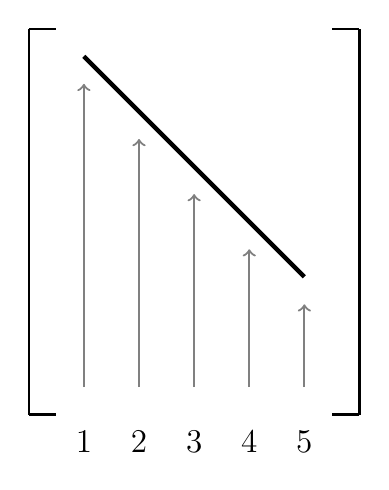
\begin{tikzpicture}[xscale=.7, yscale=.7]
    \draw[->, gray, thick](0,0)--(0,5.5);
    \draw[->, gray, thick](1,0)--(1,4.5);
    \draw[->, gray, thick](2,0)--(2,3.5);
    \draw[->, gray, thick](3,0)--(3,2.5);
    \draw[->, gray, thick](4,0)--(4,1.5);
    \node[draw=none] at(0,-1){\large 1};
    \node[draw=none] at(1,-1){\large 2};
    \node[draw=none] at(2,-1){\large 3};
    \node[draw=none] at(3,-1){\large 4};
    \node[draw=none] at(4,-1){\large 5};

    \draw[-, ultra thick] (0,6)--(4,2);

    \draw[-, thick](-1,-.5)--(-1,6.5);
    \draw[-, thick](-1, -.5)--(-.5,-.5);
    \draw[-, thick](-1,6.5)--(-.5,6.5);

    \draw[-, thick](5,-.5)--(5,6.5);
    \draw[-, thick](5,-.5)--(4.5,-.5);
    \draw[-, thick](5,6.5)--(4.5,6.5);
\end{tikzpicture}
\caption{The order in which to zero out subdiagonal entries in the Givens triangularization algorithm.
The heavy black line is the main diagonal of the matrix.
Entries should be zeroed out from bottom to top in each column, beginning with the leftmost column.}
\label{fig:Givens-iteration-order}
\end{figure}

On a $2 \times 3$ matrix, the process can be visualized as follows.
\[
\left[\begin{array}{cc}
* & * \\
* & * \\
* & * \\
\end{array}\right]
\underrightarrow{G(2,3,\theta_1)}
\left[\begin{array}{cccc}
&      *  &      *  & \\
\cline{2-3}
& \lvl{*} & \rvl{*} & \\
& \lvl{0} & \rvl{*} & \\
\cline{2-3}
\end{array}\right]
\underrightarrow{G(1,2,\theta_2)}
\left[\begin{array}{cccc}
\cline{2-3}
& \lvl{*} & \rvl{*} & \\
& \lvl{0} & \rvl{*} & \\
\cline{2-3}
&      0  &      *  & \\
\end{array}\right]
\underrightarrow{G(2,3,\theta_3)}
\left[\begin{array}{ccc}
     * &       *  & \\
\cline{2-2}
\rvl{0} & \rvl{*} & \\
\rvl{0} & \rvl{0} & \\
\cline{2-2}
\end{array}\right]
\]
At each stage, the boxed entries are those modified by the previous transformation.
The final transformation $G(2,3,\theta_3)$ operates on the bottom two rows, but since the first two entries are zero, they are unaffected.

Assuming that at the $ij$th stage of the algorithm $a_{ij}$ is nonzero, Algorithm \ref{Alg:QR-via-Givens} computes the Givens triangularization of a matrix.
Notice that the algorithm does not actually form the entire matrices $G(i,j,\theta)$; instead, it modifies only those entries of the matrix that are affected by the transformation.

\begin{algorithm}[H]
\begin{algorithmic}[1]
\Procedure{Givens Triangularization}{$A$}
\State $m, n \gets \shape{A}$
\State $R \gets \makecopy{A}$
\State $Q \gets I_{m}$
\For{$j=0\ldots n-1$}
    \For{$i=m-1\ldots j+1$}
      \State $a, b \gets R_{i-1,j}, R_{i,j}$
      \State $G \gets [[a, b],[-b,a]]/\sqrt{a^2+b^2}$
      \State $R_{i-1:i+1,j:} \gets GR_{i-1:i+1, j:}$
      \State $Q_{i-1:i+1,:} \gets GQ_{i-1:i+1,:}$
    \EndFor
\EndFor
\State \pseudoli{return} $Q\trp , R$
\EndProcedure
\end{algorithmic}
\caption{}
\label{Alg:QR-via-Givens}
\end{algorithm}

\begin{comment}
\begin{info} % Advantages and disadvantages of Givens
Like Householder transformations, Givens rotations are orthonormal, and therefore numerically stable.
In addition, they affect only a small part of the array at each iteration, making them ideal for some problems.

In general, however, Algorithm \ref{Alg:QR-via-Givens} requires more floating point operations than Algorithm \ref{Alg:QR-via-Householder}.
On the other hand, the Givens algorithm can be \emph{parallelized}, meaning that multiple processors can be used to simultaneously carry out different iterations of the algorithm.
\end{info}
\end{comment}

\subsubsection*{QR of a Hessenberg Matrix via Givens} % - - - - - - - - - - - -

The Givens algorithm is particularly efficient for computing the QR decomposition of a matrix that is already in upper Hessenberg form, since only the first subdiagonal needs to be zeroed out.
Algorithm \ref{Alg:QR-of-Hessenberg-via-Givens} details this process.

\begin{algorithm}[H]
\begin{algorithmic}[1]
\Procedure{Givens Triangularization of Hessenberg}{$H$}
\State $m, n \gets \shape{H}$
\State $R \gets \makecopy{H}$
\State $Q \gets I_{m}$
\For{$j=0\ldots \min\{n-1, m-1\}$}
    \State $i = j+1$
    \State $a, b \gets R_{i-1,j}, R_{i,j}$
    \State $G \gets [[a, b],[-b,a]]/\sqrt{a^2+b^2}$
    \State $R_{i-1:i+1,j:} \gets GR_{i-1:i+1, j:}$
    \State $Q_{i-1:i+1,:i+1} \gets GQ_{i-1:i+1,:i+1}$
\EndFor
\State \pseudoli{return} $Q\trp , R$
\EndProcedure
\end{algorithmic}
\caption{}
\label{Alg:QR-of-Hessenberg-via-Givens}
\end{algorithm}

\begin{info} % Hessenberg of Symmetric -> Tridiagonal.
When $A$ is symmetric, its upper Hessenberg form is a \emph{tridiagonal} matrix, meaning its only nonzero entries are on the main diagonal, the first subdiagonal, and the first superdiagonal.
This is because the $Q_k$'s zero out everything below the first subdiagonal of $A$ and the $Q_k\trp$'s zero out everything to the right of the first superdiagonal.
Tridiagonal matrices make computations fast, so computing the Hessenberg form of a symmetric matrix is very useful.
\end{info}
